\documentclass[tikz]{standalone}
% Rotated nodes (M4 step 7, D83 item 1, D87): a node's own rotate turns its
% shape, text and anchors about its anchor point; a scope's rotate moves nodes
% but doesn't turn them unless transform shape; positioning with rotate before
% and after the placement key; anchors and edges of a rotated node; a rotated
% label as the row lanes' titles use it.
\usetikzlibrary{positioning, fit, backgrounds, shapes.geometric}
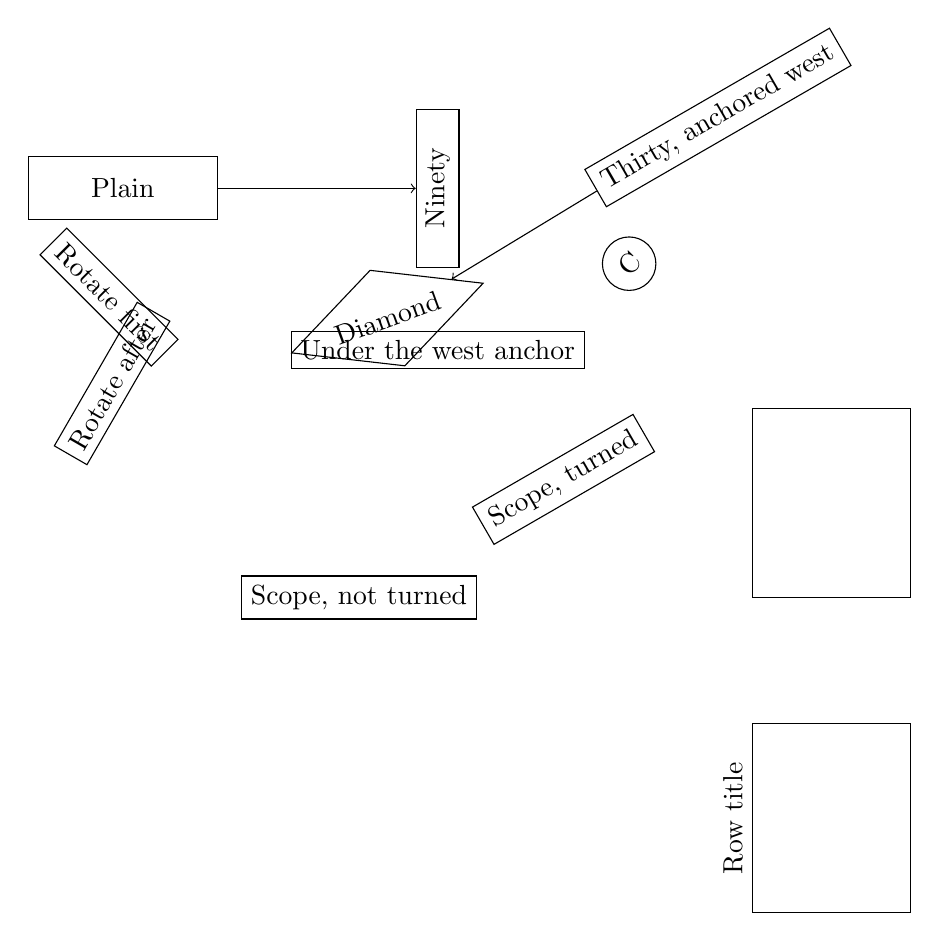
\begin{tikzpicture}[node distance=8mm and 16mm]
  \node[draw, minimum width=24mm, minimum height=8mm] (a) {Plain};
  \node[draw, rotate=90, minimum width=20mm] (r90) at (4,0) {Ninety};
  \node[draw, rotate=30, anchor=west] (r30) at (6,0) {Thirty, anchored west};
  \node[draw, rotate=-45, below=of a] (b1) {Rotate first};
  \node[draw, below=of b1, rotate=60] (b2) {Rotate after};
  \node[draw, diamond, aspect=2, rotate=20, right=of b1] (d) {Diamond};
  \node[draw, circle, rotate=45, right=of d] (c) {C};
  \node[draw, below=of r90.west] (under) {Under the west anchor};
  \coordinate (p1) at (r90.north east);
  \coordinate (p2) at (r30.east);
  \coordinate (p3) at (d.north);
  \coordinate (p4) at (r90.30);
  \draw[->] (a) -- (r90);
  \draw[->] (r30) -- (d);
  \begin{scope}[rotate=30, shift={(0,-6)}]
    \node[draw] (s1) at (0,0) {Scope, not turned};
    \node[draw, transform shape] (s2) at (3,0) {Scope, turned};
  \end{scope}
  \node[draw, minimum width=20mm, minimum height=24mm] (lane) at (9,-4) {};
  \node[draw, minimum width=20mm, minimum height=24mm,
    label={[name=t1, rotate=90, anchor=south]west:Row title}] (lane2) at (9,-8) {};
\end{tikzpicture}
